\section{Beobachter}

Für den Entwurf einer Zustandsrückführung ist es nötig, dass alle Zustandsgrössen $x$ gemessen werden können.
Dies ist oft nicht möglich oder zu teuer. \\
Stattdessen wird durch einen \textbf{Beobachter} (basierend auf dem \textbf{gemessenen Ausgangssignal} $y$) der gesamte \textbf{Zustandsvektor geschätzt}.
\textrightarrow\ Geschätzter Zustandsvektor: $\hat{x}(t)$

\smallskip

In der Struktur des Beobachter-System wird die Systemmatrix $\bm{A}$ durch die \textbf{neue Systemmatrix} $\overline{\bm{A}} = (\bm{A} - \bm{HC})$ ersetzt.
Ausserdem wird ein \textbf{Schätzfehler} $e = x - \hat{x}$ definiert, welcher gegen $0$ konvergieren soll.

\smallskip

Der Schätzfehler klingt vollständig ab, wenn der Realteil der Eigenwerte von $\overline{\bm{A}} < 0$ ist. 

\vspace{-0.2cm}

\begin{center}
    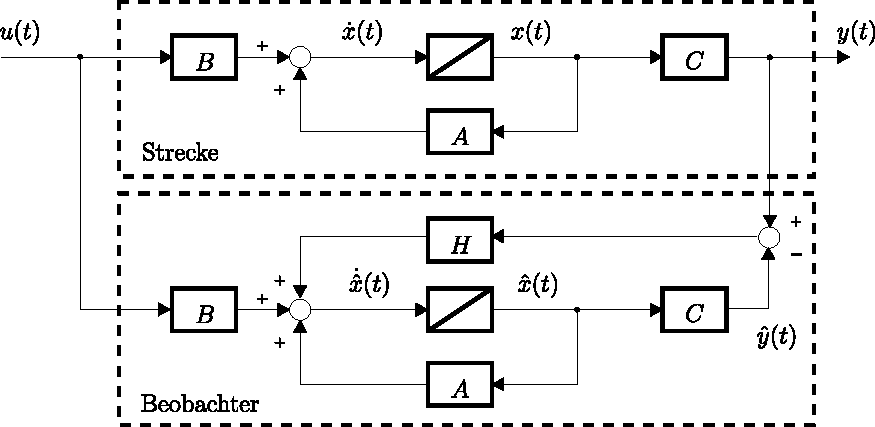
\includegraphics[width=0.85\columnwidth, align=t]{images/beobachter_strecke_mit_beobachter.pdf}
\end{center}


\textbf{Hinweis:} Für die folgenden Betrachtungen des Systems gilt $\bm{D} = 0$, sowie

\vspace{-0.1cm}

$$
\bm{H} = 
\begin{bmatrix}
        h_1 &   h_2 & \ldots    & h_n 
\end{bmatrix}^T
$$
%-----------------------------------------------------------------------------------------------------------------------------------

\para{Beobachterfehler}

\[
e=x-\hat x
\]

\[
\dot e=(A-HC)e
\]

Die Beobachterpole sind die Eigenwerte von

\[
A-HC
\]

\subsubsection{Reduzierter Beobachter}

Wird ein Teil der Zustände direkt gemessen,
müssen nur die übrigen Zustände geschätzt werden.

Anzahl Beobachterzustände:

\[
n-q
\]

mit

\[
q=
\text{Anzahl direkt gemessener Zustände}
\]

\para{Beobachter als Filter}

Kleine Beobachterverstärkung:

\[
H \downarrow
\]

\textrightarrow\ weniger Messrauschen

\textrightarrow\ langsamere Schätzung

\vspace{0.1cm}

Grosse Beobachterverstärkung:

\[
H \uparrow
\]

\textrightarrow\ schnellere Schätzung

\textrightarrow\ mehr Messrauschen
%-----------------------------------------------------------------------------------------------------------------------------------
\subsection{Dualität: Steuerbarkeit -- Beobachtbarkeit}{205}

Aufgrund der Dualität von Steuerbarkeit und Beobachtbarkeit sind viele Konzepte in den folgenden Abschnitten sehr ähnlich zu den Konzepten der Zustandsrückführung. \\
Es gelten die folgenden Korrespondenzen:

\begin{ctabular}{ccc}
    \toprule
    \textbf{Steuerbarkeit}  &               & \textbf{Beobachtbarkeit}  \\
    \midrule
    $\bm{Q_S}$              & \textlrarrow  & $\bm{Q_B^T}$              \\
    \midrule
    $\bm{B}$                & \textlrarrow  & $\bm{C^T}$                \\
    \midrule
    $\bm{A}$                & \textlrarrow  & $\bm{A^T}$                \\
    \midrule
    $\bm{K}$                & \textlrarrow  & $\bm{H^T}$                \\
    \bottomrule
\end{ctabular}


\subsection{Entwurf eines Beobachters mittels Polvorgabe}{205-207}

\textbf{Voraussetzung: Das System ist beobachtbar.} \textrightarrow\ Beobachtbarkeitsmatrix (\ref{Beobachtbarkeitsmatrix})

\smallskip

Die Ermittlung der Parameter $h_i$ des Beobachters erfolgt analog (bzw. dual) zu Ermittlung der Parameter $k_i$ der Zustandsrückführung.
Typischerweise werden die \textbf{Pole des Beobachters aber etwas weiter links} platziert (bzw. vorgegeben), damit der Fehler schneller abklingt.


\subsubsection{Vorgabe der Pollagen}

Die Eigenwerte der Matrix $\overline{\bm{A}} = (\bm{A} - \bm{HC})$ sind gegeben durch die \textbf{Wurzeln} (Nullstellen) des Polynoms

\vspace{-0.2cm}

$$ \boxed{ \det \left(\lambda \cdot \bm{I} - \overline{\bm{A}} \right) = \det \left( \lambda \cdot \bm{I} - \bm{A} + \bm{HC} \right) = (\lambda - \lambda_1) \cdot  (\lambda - \lambda_2) \ldots  (\lambda - \lambda_n) } $$

Die Eigenwerte von $\overline{\bm{A}} = (\bm{A} - \bm{HC})$ müssen mit den \cbl{vorgegebenen Polen} übereinstimmen.
Dies wird wieder durch einen \textbf{Koeffizientenvergleich} erreicht.

\vspace{-0.2cm}

$$ \boxed{ \cbl{(s - p_1) \cdot (s - p_2) \cdot \ldots \cdot (s - p_n)} \overset{!}{=}
\det \left( s \cdot \bm{I} - \bm{A} + \bm{HC} \right) } $$

% \textbf{Hinweis:} Die Parameter $h_i$ sind \textbf{eindeutig} bestimmbar, sofern das System \textbf{beobachtbar} ist.


\subsubsection{Separationsprinzip}

In der Regelungstechnik werden oft Systeme mit Zustandsrückführung \textbf{und} Beobachter eingesetzt. 

\begin{center}
    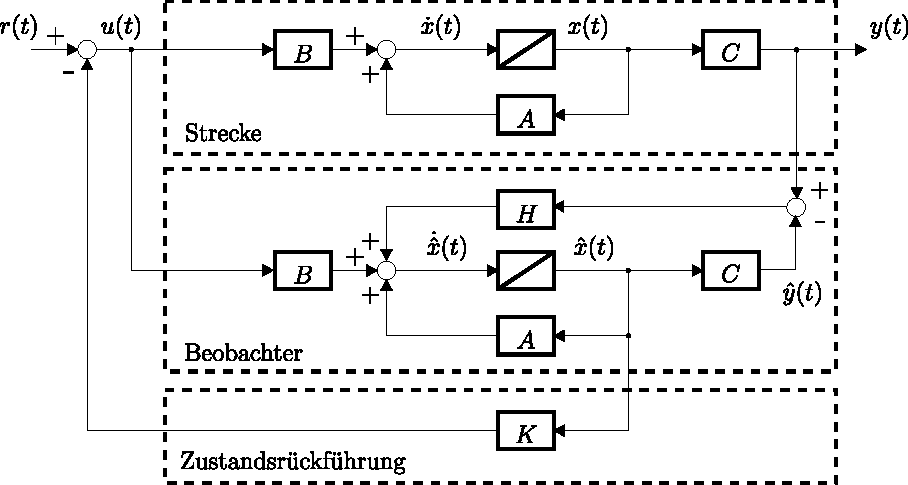
\includegraphics[width=0.85\columnwidth, align=t]{images/beobachter_strecke_beobachter_ZRF.pdf}
\end{center}

Es kann gezeigt werden, dass beide Teilsysteme (Zustandsrückführung und Beobachter) \textbf{separat entworfen} werden können und ein \textbf{stabiles Gesamtsystem} resultiert. \\
Die Bedingungen dafür sind:

\begin{tabular}{ll}
    \tabitem Zustandsrückführung stabil:    & $\det(\lambda_Z \cdot \bm{I} - \bm{A} + \bm{BK}) \overset{!}{=} 0 \quad \rightarrow \forall \lambda_Z \quad \mathrm{Re} \{ \lambda_Z \} < 0$ \\
    \tabitem Beobachter stabil:             & $\det(\lambda_B \cdot \bm{I} - \bm{A} + \bm{HC}) \overset{!}{=} 0 \quad \rightarrow \forall \lambda_B \quad \mathrm{Re} \{ \lambda_B \} < 0$
\end{tabular}

\medskip

Die Eigenwerte (bzw. Pole) des Gesamtsystems entsprechen der \textbf{Vereinigung der Eigenwerte der Teilsysteme}.
Die Eigenwerte (bzw. Pole) könnten auch durch Lösung einer einzigen (aufwendigen) Gleichung gelöst werden:

\vspace{-0.2cm}

$$ \det(\lambda \cdot \bm{I} - \bm{A} + \bm{BK}) \cdot \det(\lambda \cdot \bm{I} - \bm{A} + \bm{HC}) \overset{!}{=} 0 $$

\textbf{Hinweis:} Gezeigt ist die 'Eigenwert-Sicht'. Wenn gezeigt werden soll, dass der Fokus auf den Polen liegt, dann wird in den Gleichungen jeweils $\lambda$ durch $s$ ersetzt.


\subsection{LQG-Verfahren (Linear Quadratic Gaussian Estimation)}

Die duale Methode zum LQR-Verfahren der Zustandsrückführung ist das LQG-Verfahren.
Im Gegensatz zum LQR-Verfahren handelt es sich beim LQG-Verfahren um ein \textbf{stochastisches Optimierungsproblem}.


\subsubsection{Optimale Beobachterverstärkung $\bm{H}$}

Die optimalen Beobachterverstärkungen (als Matrix $\bm{H}$) ergeben sich aus der positiv definiten Lösung der Matrix $\bm{S}$ der entsprechenden Matrix-Ricatti-Gleichung:

\vspace{-0.2cm}

$$ \boxed{ \bm{H} = (\bm{R^{-1} C S})^T = \bm{S C^T R^{-1}} } $$

\textbf{Hinweis:} Meist wird die Lösung $\bm{H}$ direkt mit Matlab ermittelt.


\subsubsection{Eigenschaften des LQG-Verfahrens}

\begin{outline}
    \1 Die Gewichtungsmatritzen $\bm{R}$ und $\bm{Q}$ werden \textbf{positiv definit} gewählt
        \2 Die Gewichtungsmatritzen charakterisieren die Rauschleistung im System
    \1 Ist $\bm{R}$ klein, so ist das Messrauschen gering bzw. die Messung zuverlässig
        \2 Die Verstärkung $\bm{H}$ ist dann grösser und Regelkreis somit schneller
    \1 Die Robustheit des Gesamtsystems ist \textbf{nicht garantiert}, wenn Beobachter und Zustandsrückführung \textbf{unabhängig voneinander} entworfen werden
        \2 Separationsprinzip gilt nicht für Robustheit bei LQG!
\end{outline}


\subsection{Varianten von Beobachtern}{209-211}

\subsubsection{Beobachter für Teilsysteme}

Ein Beobachter kann auch den Ausgang eines Teilsystems (hier $w$) beobachten, statt den Ausgang des Gesamtsystems.
Auch muss der Eingang eines Beobachters nicht der Stellgrösse $u$ entsprechen, sondern kann das Ausgangssignal eines vorherigen Teilsystems sein (hier $w$).

\vspace{-0.2cm}

\begin{center}
    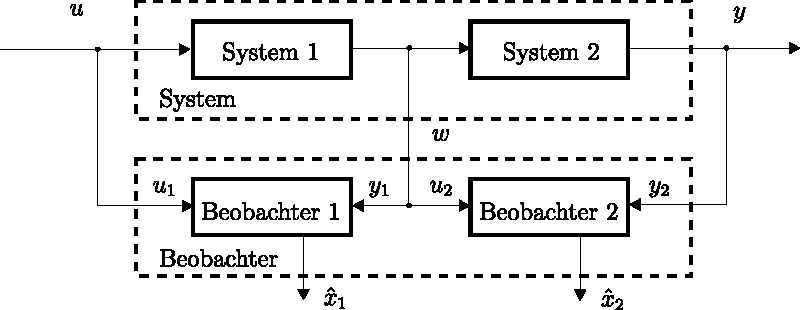
\includegraphics[width=0.8\columnwidth]{images/beobachter_teilsysteme.pdf}
\end{center}

\vspace{-0.2cm}

Durch die Beobachtung von Teilsystemen kann die \textbf{Komplexität beim Entwurf reduziert} werden.


\subsubsection{Redundante Messungen}

Redundante Messungen sind sinnvoll, wenn Messrauschen vorhanden ist.

\smallskip

Zwei Sensoren, welche unabhängig voneinander dieselbe Grösse messen, liefern dasselbe Signal, überlagert von unterschiedlichem Rauschen.
Das Signal kann mit zwei Sensoren besser geschätzt werden, wobei natürlich eine Kosten-Nutzen-Rechnung gemacht werden muss.



\subsubsection{Reduzierter Beobachter}

Wenn Zustandsgrössen rauschfrei gemessen werden können, ist es nicht nötig, diese zu schätzen. 
Es müssen dann nur $n - \mu$ Grössen geschätzt werden. Somit kann der Beobachter reduziert werden.

\smallskip

Bei folgender Darstellung der ZRD des Beobachters wird angenommen, dass die \textbf{Messgrössen einem Teil des Zustandsvektors entsprechen}.
Diese müssen folglich \textbf{nicht} durch den Beobachter geschätzt werden.

\vspace{-0.1cm}

\begin{minipage}[c]{0.5\columnwidth}
    \begin{align*}
        \begin{bmatrix} \dot{x}_{\nu} \\ \dot{x}_{\mu} \end{bmatrix}    &= \begin{bmatrix} \bm{A_{11}}   & \bm{A_{12}} \\ \bm{A_{21}}  & \bm{A_{22}} \end{bmatrix} \cdot \begin{bmatrix} x_{\nu} \\ x_{\mu} \end{bmatrix}
                                                                        + \begin{bmatrix} \bm{B_1} \\ \bm{B_2} \end{bmatrix} \cdot u                                                                                        \\
        y                                                               &= \begin{bmatrix} \bm{0} & \bm{I} \end{bmatrix} \cdot \begin{bmatrix} x_{\nu} \\ x_{\mu} \end{bmatrix}
    \end{align*}
\end{minipage}
\hfill
\begin{minipage}[c]{0.45\columnwidth}
    \begin{tabular}{ll}
        $x_{\mu}$   & gemessene Zustandsgrössen     \\
        $x_{\nu}$   & geschätzte Zustandsgrössen    \\
    \end{tabular}
\end{minipage}

\smallskip

\paragraph{Realisierung des reduzierten Beobachters}

\begin{center}
    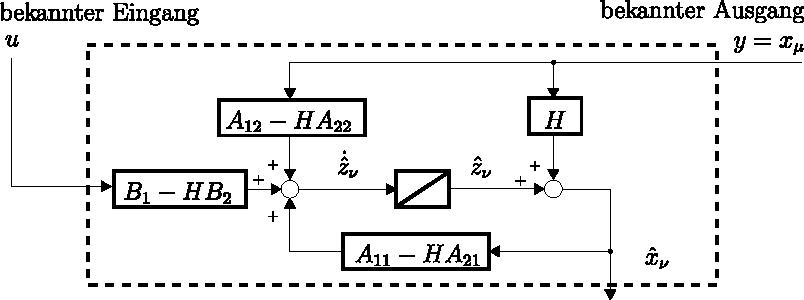
\includegraphics[width=0.8\columnwidth, align=t]{images/beobachter_reduziert.pdf}
\end{center}

\vspace{-0.2cm}


\subsection{Implementierung eines Zustandsreglers mit Beobachter}

Für eine SISO-Strecke wurde ein Zustandsregler mit Beobachter mit Verstärkung $k$ und eine Vorverstärkung $L$ entworfen.

\vspace{-0.2cm}

\begin{center}
    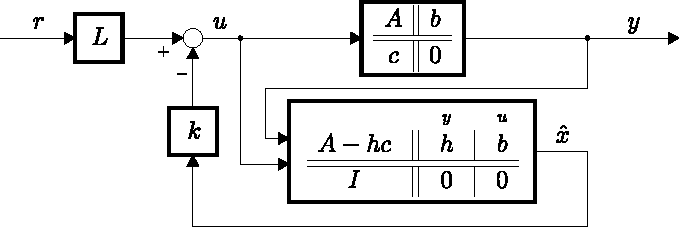
\includegraphics[width=0.8\columnwidth, align=t]{images/beobachter_zustandsregler_vorverstaerkung.pdf}
\end{center}


Das System kann auch so betrachtet werden, dass der Beobachter und die Vorverstärkung mit in den Regler 'gepackt' werden.
Durch einsetzen von $u = L r - k \hat{x}$ (gemäss Regelkreis oben) ergibt sich für das Gesamtregelsystem (unten) die folgende ZV-Darstellung:

\begin{ctabular}{r c c c c c}
    $\dot{\hat{x}} =$   & $(\bm{A}- hc - bk)$   & $\hat{x} \ +$ & $bLr$   & $+ \ hy$  \\
    $u =$               & $-k$                  & $\hat{x} \ +$ & $Lr$    &           \\
\end{ctabular}

\begin{center}
    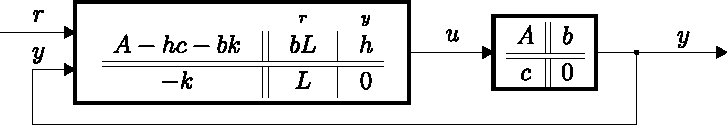
\includegraphics[width=0.8\columnwidth, align=t]{images/beobachter_zustandsregler_gesamtsystem.pdf}
\end{center}

\vspace{-0.2cm}


\subsubsection{Eigenschaften der Implementierung}

\begin{outline}
    \1 Gesamtregler ist MIMO-System mit Eingängen $r$ und $y$
    \1 Die beiden UTF $\frac{U(s)}{R(s)}$ und $\frac{U(s)}{Y(s)}$ haben dieselbe Systemmatrix $(\bm{A} - hc - bk)$
        \2 Beide UTF haben somit \textbf{identische Pole}
        \2 Nullstellen der beiden UTF sind unterschiedlich
\end{outline}

\vspace{-0.4cm}

$$ \frac{U(s)}{R(s)} = \frac{\beta_n s^n \beta_{n-1} s^{n-1} + \cdots + \beta_1 s + \beta_0}{s^n + \alpha_{n-1} s^{n-1} + \cdots + \alpha_1 + \alpha_0} \qquad \quad
    \frac{U(s)}{Y(s)} = \frac{\overline{\beta}_m s^m \overline{\beta}_{m-1} s^{m-1} + \cdots + \overline{\beta}_1 s + \overline{\beta}_0}{s^n + \alpha_{n-1} s^{n-1} + \cdots + \alpha_1 + \alpha_0} $$


\subsubsection{Reglerstruktur -- Zustandsreglers mit Beobachter}

Die folgende Filterform (Direkte Form) implementiert die \textbf{minimale Realisierung} des Reglers mit Beobachter.
Es sind allerdings auch andere Realisierungen möglich.

\vspace{-0.2cm}

\begin{center}
    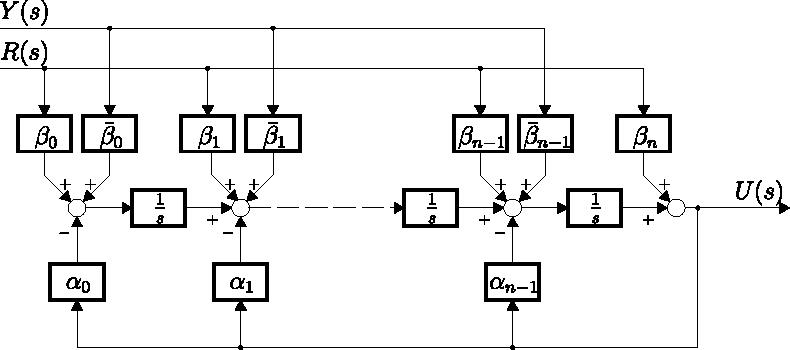
\includegraphics[width=0.8\columnwidth, align=t]{images/beobachter_implementation.pdf}
\end{center}

